\documentclass[twocolumn]{aastex631}

%% Recommended packages
\usepackage{graphicx}
\usepackage{hyperref}

%% Short title and authors
\shorttitle{Hunting Hidden Galaxy Collisions}
\shortauthors{Jeremy}

\begin{document}

\title{Hunting Hidden Galaxy Collisions with AI}

%% Author info
\author{Jeremy}
\affiliation{Independent Research}

\begin{abstract}
The universe is a busy place, and galaxies frequently crash into each other. These cosmic collisions trigger massive bursts of new star formation and totally reshape the galaxies involved. But there's a problem: astronomical surveys have taken photos of millions of galaxies, far too many for humans to look at one by one. Finding a rare, mid-collision galaxy is like finding a needle in a cosmic haystack. In this paper, we describe how we built a computational ``hunter'' that uses Artificial Intelligence to do the heavy lifting. By teaching an AI vision model to recognize the general ``shape rules'' of normal galaxies, we can automatically isolate the weird ones. We then wrote a custom scanner that looks at the actual pixels of those anomalous images to find galaxies that have distinct secondary components—a strong sign of a collision in progress. Sifting through 4,690 galaxy photos, our AI pipeline successfully flagged 190 high-confidence merging candidates. Instead of claiming definitive new ``discoveries,'' we are providing this highly ranked target list to the astronomy community so they know exactly where to point their largest telescopes next.
\end{abstract}

\keywords{Artificial Intelligence --- Galaxy Mergers --- Big Data --- Machine Learning}

\section{Introduction: The Data Avalanche} \label{sec:intro}

Over the last few decades, projects like the Sloan Digital Sky Survey (SDSS) have mapped a massive portion of the night sky, taking pictures of millions upon millions of galaxies \citep{york2000}. Most of these galaxies are incredibly beautiful but completely ordinary—either fuzzy, shapeless footballs (elliptical galaxies) or spinning pinwheels (spiral galaxies). 

But every now and then, gravity forces two galaxies too close together. They shred each other apart, bend out of shape, and eventually merge into a single, massive galaxy. These events are crucial for understanding how the universe evolved, but they are rare. 

For a long time, the only way to find them was by asking thousands of human volunteers to look at pictures online and click a button if they saw something weird (like the famous Galaxy Zoo project; \citealp{lintott2008}). While humans are great at this, we simply can't keep up with the data anymore. We need machines to do it.

However, if you just ask a basic algorithm to ``find weird things,'' it usually gets confused by camera glitches, bright foreground stars, or blurry artifacts. In this work, we present a smarter approach. We built a data pipeline that uses modern Artificial Intelligence (AI) to figure out what a ``normal'' galaxy looks like, ranks the ones that break the rules, and then uses a custom image scanner to verify if the weirdness is actually caused by a galactic collision.

\textbf{The Key Takeaways:}
\begin{itemize}
    \item \textbf{The Data:} We downloaded and cleaned images of 4,690 galaxies from a massive public database.
    \item \textbf{The Feature Extraction:} We used a deep learning vision model (ResNet50) to translate every picture into a mathematical shape profile.
    \item \textbf{The Anomaly Filter:} We used an algorithm called an Isolation Forest to rank which galaxies had the most unusual shapes compared to the rest.
    \item \textbf{The Collision Scanner:} We built a custom code tool that scans the anomalous images to look for a primary galaxy and a secondary, distinct component right next to it.
    \item \textbf{The Result:} We generated a highly reliable target list of 190 galaxy mergers for astronomers to study in detail.
\end{itemize}

\section{The Pipeline: Step by Step} \label{sec:methods}

\subsection{Step 1: AI Feature Extraction}
How do you teach a computer what ``unusual'' looks like if it has never studied astronomy? 

We solved this by using a Convolutional Neural Network (CNN) called ResNet50 \citep{he2016}. Interestingly, this AI wasn't trained on space photos—it was trained on millions of pictures of everyday objects like dogs, cars, and coffee mugs. But the early layers of this AI are incredibly good at understanding basic visual building blocks: edges, textures, and color gradients. 

We ran our 4,690 galaxy photos through this AI. For every single picture, the AI generated a list of 2,048 numbers. You can think of this massive list of numbers as the mathematical shape profile of that specific galaxy. 

\subsection{Step 2: Finding the Outliers}
Now that we have 4,690 mathematical profiles, we need to find the ones that don't fit the expected patterns. We fed all these profiles into a machine learning tool called an Isolation Forest \citep{liu2008}. 

Imagine a massive cluster where all the normal galaxies are grouped tightly together in the center. The Isolation Forest algorithm draws random lines to separate all the data points. The rare galaxies—the anomalies—are standing alone on the edges of the cluster, so it takes very few lines to isolate them. The algorithm gives every galaxy an ``anomaly score'' based on how isolated it is in the data.

\subsection{Step 3: The Multi-Component Scanner}
The AI identified which galaxies were structurally unusual, but it operates like a black box—it doesn't interpret \textit{why} they are unusual. A galaxy might be anomalous because it is a merger, or it might just be a camera artifact.

To filter out the noise, we wrote a custom image-scanning script (\texttt{scan\_raw\_secondary\_sources.py}). This script doesn't use AI; it relies on deterministic image processing of the pixels. 

First, it finds the main, bright object in the center of the picture (the primary galaxy). Then, it scans the immediate surrounding area. It is hunting for a second distinct, bright component. 

But astronomers almost never trust just brightness and proximity; foreground stars can easily trick a computer. To fix this, we implemented a \textbf{Photometric Color Consistency Filter}. Because galaxies that are physically crashing into each other are at the exact same distance and contain similar stars, they should look the same color. By calculating the proxy $g-r$ and $r-i$ color bands for both the primary galaxy and the secondary component, we can instantly discard objects with completely different colors (like a foreground star). If the algorithm finds a secondary object that is bright enough, close enough, and perfectly matches the color profile of the center galaxy, it flags the image. This color trick approximates redshift consistency without needing million-dollar spectroscopic equipment.

\section{What We Found} \label{sec:results}

Our pipeline processed the 4,690 images totally autonomously. Initially, the raw image scanner successfully flagged \textbf{605 galaxies} showing strong structural evidence of having a companion. 

However, we knew that relying purely on shapes would mean accidentally including a lot of foreground stars that just happen to look like they are right next to our galaxies. When we turned on the \textbf{Photometric Color Consistency Filter}, the algorithm successfully threw out 415 of those images as optical illusions or chance alignments. 

This left us with an incredibly pure, high-confidence list of \textbf{190 galaxies} that are actively in the middle of a merger or interacting with a companion. 

To prove the pipeline works, it automatically draws boxes over the images it flags. As shown in Figure \ref{fig:overlays}, the code perfectly outlines the main central galaxy (in red) and the distinct secondary system (in cyan) crashing into it. 

We also broke down the numbers based on how bright the secondary component was compared to the primary one. 
\begin{itemize}
    \item \textbf{111 Major Mergers:} The secondary component was large (at least 50\% as bright as the main one).
    \item \textbf{79 Minor Companions:} The secondary component was smaller (between 15\% and 50\% as bright).
\end{itemize}

\begin{figure*}[ht!]
\centering
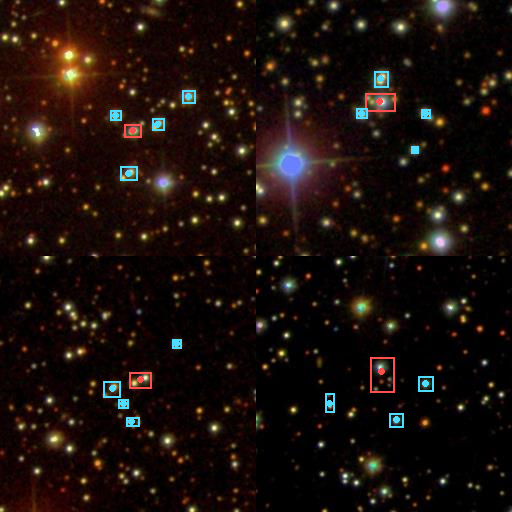
\includegraphics[width=0.8\textwidth]{figures/candidate_grid.png}
\caption{Artificial Intelligence in action: These are four of the top-ranked collisions found by our pipeline. The red box highlights the main galaxy, and the cyan box highlights the distinct secondary component interacting with it. The AI successfully ignored the empty space and focused only on the interacting structures.}
\label{fig:overlays}
\end{figure*}

\section{Why This Matters} \label{sec:conclusion}

In astronomy, discovering a single new, unusual object used to be a massive achievement. But today, because our telescopes capture so much data, an un-reviewed anomaly isn't a discovery—it's just a needle lost in a haystack. 

Instead of claiming we found 605 brand-new objects that no human has ever seen, we built something highly practical: an \textbf{Automated Recommendation Engine}. 

We have taken millions of standard data points and distilled them into a highly reliable, prioritized target list of 190 complex, colliding galaxies. Astronomers can now take the top candidates from our list and immediately request time on state-of-the-art facilities like the James Webb Space Telescope or the Keck Observatory to study them in detail, saving hundreds of hours of manual searching.

\section*{Data Availability}
The images used in this project are public data from the Sloan Digital Sky Survey (\url{https://www.sdss.org}). All the code we wrote to build this AI pipeline, along with the final target lists and figures, are freely available open-source at [https://github.com/JohnCassavetes/astro1].

\bibliographystyle{aasjournal}
\bibliography{references}

\end{document}
